\documentclass[a4paper, 12pt]{article}%тип документа

%отступы
\usepackage[left=1.5cm,right=1cm,top=2cm,bottom=3cm,bindingoffset=0cm]{geometry}
\setlength{\parindent}{5ex}
%Русский язык
\usepackage[T2A]{fontenc} %кодировка
\usepackage[utf8]{inputenc} %кодировка исходного кода
\usepackage[english,russian]{babel} %локализация и переносы

%Вставка картинок
\usepackage{graphicx}
\graphicspath{{pictures/}}
\DeclareGraphicsExtensions{.pdf,.png,.jpg,}
\usepackage{wrapfig}

%Графики
\usepackage{pgfplots}
\pgfplotsset{compat=1.9}

%Математика
\usepackage{amsmath, amsfonts, amssymb, amsthm, mathtools}

%Таблицы
\usepackage{longtable} 
\usepackage{float}

%Римские цифры
\newcommand{\RomanNumeralCaps}[1]{\uppercase\expandafter{\romannumeral#1}}

\usepackage{multirow}



\begin{document}
	\begin{titlepage}
		\begin{center}
			\textsc{Федеральное государственное автономное образовательное учреждение высшего образования«Московский физико-технический институт (национальный исследовательский университет)»\\[5mm]
			}
			
			\vfill
			
			\textbf{Отчёт по лабораторной работы 4.3.2\\[3mm]
				Дифракция когерентного излучения на шероховатой поверхности.
				\\[50mm]
			}
			
		\end{center}
		
		\hfill
		\begin{minipage}{.5\textwidth}
			Выполнил студент:\\[2mm]
			Сериков Василий Романович\\[2mm]
			группа: Б03-102\\[5mm]
			
		\end{minipage}
		\vfill
		\begin{center}
			Москва, 2023 г.
		\end{center}
		
	\end{titlepage}
	
	\newpage
	\setcounter{page}{2}
	\textbf{Аннотация}\\
	
	\textbf{Цель работы: }\\
	
	Получение и исследование изображений стохастических дифракционных полей (спеклов), приобретение навыков обработки двумерных цифровых сигналов.\\
	
	\textbf{В работе используются:}\\
	
	 Гелий-неоновый лазер, матовая пластинка, поляроид, цифровая камера, компьютер.\\
	 
	 
	 \textbf{Теория: }\\
	 
	 \begin{figure}[H]
	 	\center{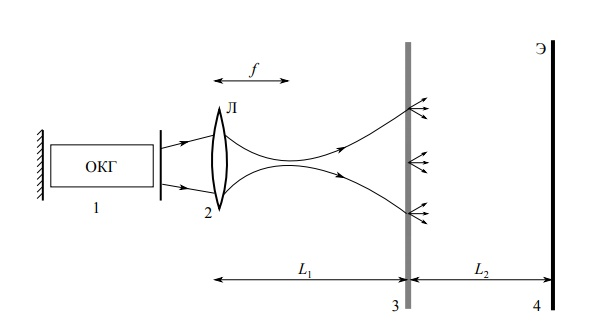
\includegraphics[scale=0.9]{scheme.jpg}}
	 	\caption{Схема получения спекл-картины: 1 — гелий-неоновый лазер, 2 — линза, 3 — рассеиватель, 4 — экран или фотокамера}
	 \end{figure}
	
	
	Источником излучения служит He–Ne-лазер с длиной волны излучения 0,63 мкм. Пучок излучения, формируемый линзой, рассеивается на
	матовой стеклянной пластинке, на экране наблюдается спекл-картина
	рассеяния. В простых экспериментах можно исследовать зависимость спекл-картины от
	поперечного размера лазерного луча на рассеивателе: чем «острее» фокусировка, тем более крупные спеклы возникают на экране, и, наоборот,
	увеличение диаметра луча приводит к уменьшению размеров спеклов.
	При увеличении расстояния L2 между рассеивателем и экраном спеклы
	увеличиваются в размере.
	
	Из качественного описания ясно, что вид спекл-картины определяется возмущениями фронта световой волны, вносимыми шероховатой
	рассеивающей поверхностью. Возмущения волнового фронта создаются случайной функцией h(x, y), поэтому для анализа этих возмущений
	необходимо использовать статистические методы.
	
	Гелий-неоновый лазер генерирует слабо расходящийся пучок
	света на длине волны $\lambda$ = 0,63 мкм. Можно принять, что на выходе
	из лазера пучок имеет плоский волновой фронт, а распределение
	интенсивности света в пучке описывается гауссовой функцией:
	
	\begin{equation}
		I_L(\boldsymbol{r})=\left|E_L(\boldsymbol{r})\right|^2=I_0 e^{-\frac{r^2}{\rho_L^2}},
	\end{equation}

где   $\rho_L$ — поперечное расстояние от оси лазерного луча, на котором интенсивность уменьшается в e раз по сравнению с максимальной. На выходе лазера $\rho_L \approx$  100 мкм. Как известно, при распространении гауссова
пучка его поперечный размер $\rho_l$ увеличивается, но форма сохраняется. Линза, показанная на рис. 1, изменяет размер пучка, но не меняет
его гауссовой формы. Матовая пластинка, стоящая на пути лазерного
луча, вносит поперечную неоднородность в световое поле и значительно
увеличивает угловую расходимость пучка. Когерентное лазерное излучение преобразуется матовой поверхностью в поперечно-некогерентное.
	
Согласно определению, корреляционной функцией $\Psi$ является функция

\begin{equation}
	\Psi_h(\rho)=\langle h(r) h(r+\rho)\rangle-\langle h(r)\rangle^2
\end{equation}

где $\rho$ - смещение относительно точки $r$, скобки <..> означают усреднение по всем точкам поверхности. Функция показывает, насколько в среднем изменяется величина $h$. при смещении из данной точки на расстояние $\rho$, Другими словами, насколько значение $h(r)$ и $h(r+\rho)$ скоррелированы между собой. Для однородной пластинки функция $\Psi$ не зависит оп выбора точки $r$, а определяется только величиной смещения $\rho$, т. е. $\Psi_h=\Psi_h(\rho)$. Общие соображения позволяют представить качественно вид функции $\Psi h(\rho)$. При $\rho=0$ значения $h(\boldsymbol{r})$ и $h(\boldsymbol{r}+\rho)$ одинаковы, т. e. их корреляция наибольшая, а функция $\Psi_h(\rho)$ достигает максимума (в этом случае $\Psi_h(\rho)=\left\langle h^2(r)\right\rangle-(\ell(r))^2=\sigma_h^2$, согласно определению дисперсии). При больших значениях $\rho$ в силу случайного характера функции $b$ значения $h(r)$ п $h(r+p)$ оказываются независимыми и функция $\Psi(p) \rightarrow 0$. Таким образом, функция $\Psi_h(p)$ должна достигать максимального значения при $\rho=0 \mathrm{~s}$ уменьшаться с ростом $\rho$. Обычно хорошим приближением дли корреляционной функции $\Psi_h(\rho)$ является функция Гауcca:
$$
\Psi h(p)=\sigma_{h,}^2 e^{-\frac{\Delta^2}{p_h^2}}
$$
где $\rho_h$ - характерное расстояние, называемое радиусом корреляции, на
котором функция корреляции уменьшается в e раз.\\

	
	
\textbf{Ход работы: }\\
	\begin{enumerate}
		\item Получим изображения спеклов, полученных через матовую пластинку. По полученным фотографиям рассчитаем с помощью программы «Индикатриса»  следующие параметры: радиус индикатрисы рассеяния $\rho_h$, параметр шероховатости $\zeta$.
		
			$$ \rho_h = d\cdot m $$
		
		$$
		\zeta:=\frac{\rho_h}{2 \cdot L_2 \cdot\left(n_\lambda-1\right)}, \text{   } n_\lambda = 1,5 \text{ - показатель преломления стекла}
		$$
		
		\newpage
		
		\begin{longtable}{|c|c|c|c|c|c|}
			\hline
			$L_1$, мм  & $L_2$, мм  & m, пиксель& $\rho_h$, мм   & $\zeta$   & d, мм  \\ \hline
			20  & 20  & 493 & 2,317 & 0,116 & \multirow{2}{*} {4,7$\cdot 10^{-3}$ }\\ \cline{1-5}
			30  & 20 & 514 & 2,416 & 0,121 &  \\ \hline
			\caption{Полученные значения $\rho_h$ и $\zeta$}
		\end{longtable}
		
		
		
	\item С помощью программы "Корреляция" узнаем радиус корреляции $\rho_c$ и оценим радиус лазерного пучка $\rho_L$ по полученным данным.
	
	$$ \rho_L = \frac{\lambda L_2}{\sqrt{2} \pi \rho_c}, \lambda = 630\text{нм} $$
	
	\begin{longtable}{|c|c|c|c|c|}
		\hline
		$L_1$, мм  & $L_2$, мм  & m, пиксель& $\rho_c$, мм& d, мм  \\ \hline
		20  & 20  & 4 & 0,019 & \multirow{7}{*} {4,7$\cdot 10^{-3}$ }\\ \cline{1-4}
		20  & 40  & 7 & 0,033 &  \\ \cline{1-4}
		20  & 60  & 10 & 0,047 &  \\ \cline{1-4}
		20  & 80  & 13 & 0,061 &  \\ \cline{1-4}
		30  & 20  & 3 & 0,014 &  \\ \cline{1-4}
		30  & 40  & 6 & 0,028 &  \\ \cline{1-4}
		30  & 60  & 8 & 0,038 &  \\ \hline
		% 30  & 80 & 514 & 2,416 &   \\ \hline
		\caption{Полученные значения $\rho_c$}
		
		
	\end{longtable}
	
		\begin{figure}[H]
			\center{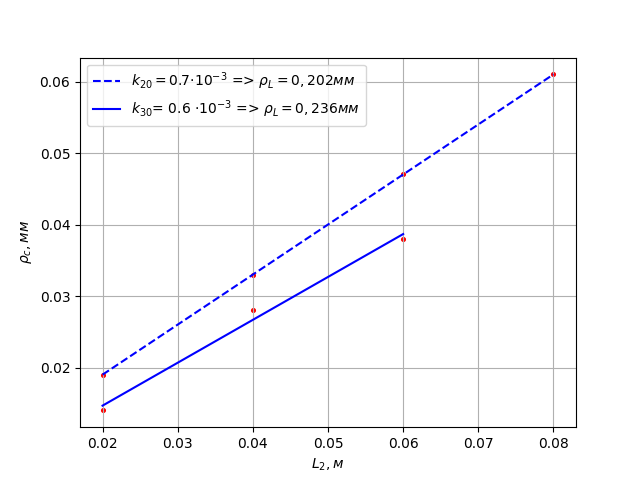
\includegraphics[scale=0.9]{rho(L).png}}
			\caption{График зависимости $\rho_c(L_2)$ и значения радиуса лазерного пучка}
		\end{figure}
	
	\end{enumerate}
	
	

	
	\textbf{Обсуждение результатов и выводы: }\\
	
	В ходе данной работы мы познакомились с явлением дифракции на шероховатой поверхности, получили картины спеклов и по ним с помощью программного обеспечения mathcad определили параметр шероховатости поверхности, рассчитали радиус лазерного пучка, определили радиусы корреляции и индикатрисы рассеяния.
	
	
	
	
	
	
	
	
	
	
	
	
	
	
	
	
	
	
	
	
	
	
	
	
	
	
	
	\end{document}